\section{Neutrino Oscillations and Interactions}
\label{sec:Theory}

Neutrinos are neutral, spin 1/2 fermions that have only been observed with left-handed chirality. There are three types of neutrinos, $\nu_e$, $\nu_\mu$ and $\nu_\tau$ each corresponding with one of the Standard Model (SM) leptons. They are produced via weak interactions and are always observed in one of these three flavors. According to the SM, these neutrinos are also massless; a prediction that has been found incorrect in the recent decades as a direct implication of the phenomenon of neutrino oscillation. Also if the energies are known, neutrinos provide a way to measure the axial form factors that describe the internal structure of a nucleon. In the following sections, we calculate various observable quantities of interest in neutrino science including the probabilities of oscillation and three major neutrino-nucleon scattering cross sections.

\subsection{Neutrino Mixing}
\label{sec:neutosc}

Observations from solar, atmospheric and reactor neutrino experiments suggested that while a neutrino is produced as one of three flavors, over time and distance they oscillate into another. This manifests in experiments as an excess of an unexpected neutrino flavor (\emph{appearance}) or as a deficit in the expected neutrino flavor (\emph{disappearance}). The ability for neutrinos to oscillate into a different flavor state implies that neutrinos do in fact have mass, albeit a small one. It also implies that each flavor state is also a linear superposition of three different mass states. This observation is called neutrino mixing. Experimental measurement of the invisible $Z^0$ decay width confirms that there are only 3 neutrinos flavors that couple with the Z boson.

As neutrinos are electrically neutral, it is unknown whether neutrinos are Dirac or Majorana particles. In the three neutrino picture, the unitary matrix ($U$) describing the mixing of the states has three Euler angles and six phases. If neutrinos are Dirac particles, then only one complex phase has a physically observable effect and is called the Dirac CP violating phase $\delta_{CP}$. However, if neutrinos are Majorana particles, then there are three CP violating phases. In this case, the unitary mixing matrix can be decomposed to the form
\begin{equation}
U = V P
\end{equation}
where V contains all the Dirac angles and phases and P contains the additional Majorana phases. The Majorana phases do not contribute to the phenomenon of neutrino mixing, so we ignore them. We will only consider the Dirac part of the mixing matrix and, to simplify the notation, henceforth call it $U$.

In the three neutrino picture, assuming that the three mass states are not degenerate (i.e. $m_1 \neq m_2 \neq m_3$), the fact that the flavor states are linear combinations of mass states can be represented by
\begin{equation}
\ket{\nu_\alpha} = \sum_i U^*_{\alpha i} \ket{\nu_i}.
\end{equation}
Here, $\ket{\nu_\alpha}$ is a flavor eigenstate, $\ket{\nu_i}$ is a Hamiltonian eigenstate and $U^*$ is the unitary Dirac mixing matrix
\begin{equation}\label{eq:U}
\begin{aligned}
U &= \begin{pmatrix}
1 & 0 & 0 \\
0 & c_{23} & s_{23} \\
0 & -s_{23} & c_{23} \end{pmatrix}
\begin{pmatrix}
c_{13} & 0 & s_{13} e^{-i \delta} \\
0 & 1 & 0 \\
-s_{13} e^{i \delta} & 0 & c_{13} \end{pmatrix}
\begin{pmatrix}
c_{12} & s_{12} & 0 \\
-s_{12} & c_{12} & 0 \\
0 & 0 & 1 \end{pmatrix}
%\begin{pmatrix}
%1 & 0 & 0 \\
%0 & e^{i \alpha_{1}/2} & 0 \\
%0 & 0 & e^{i \alpha_{2}/2} \end{pmatrix} 
\\
& = \begin{pmatrix}
c_{12} c_{13} & s_{12} c_{13} & s_{13} e^{-i \delta} \\
-s_{12} c_{23} - c_{12} s_{23} s_{13} e^{i \delta} & c_{12} c_{23} - s_{12} s_{23} s_{13} e^{i \delta} & s_{23} c_{13} \\
s_{12} s_{23} - c_{12} c_{23} s_{13} e^{i \delta} & -c_{12} s_{23} - s_{12} c_{23} s_{13} e^{i \delta} & c_{23} c_{13} \end{pmatrix}
%\begin{pmatrix}
%1 & 0 & 0 \\
%0 & e^{i \alpha_{1}/2} & 0 \\
%0 & 0 & e^{i \alpha_{2}/2} \end{pmatrix}.
\end{aligned}
\end{equation}
 In vacuum, the Hamiltonian eigenstates, $\lambda_i$, are just the vacuum energy eigenstates, so the time evolution of the flavor state is given by
\begin{equation}
\ket{\nu_\alpha(t)} = \sum_i U_{\alpha i}^*e^{-i\lambda_i t}\ket{\nu_i}.
\end{equation}
The neutrino oscillation amplitude after some time $t$, given that mass eigenstates are orthogonal, is then
\begin{align}
\braket{\nu_\beta|\nu_\alpha(t)} &= \left(\sum_j \bra{\nu_j}U^T_{j\beta}\right)\left( \sum_i U_{\alpha i}^*e^{-i\lambda_i t}\ket{\nu_i}\right)\\
&= \sum_i U^*_{\alpha i} e^{-i\lambda_i t} U_{\beta i}.
\end{align}
Squaring this yields the oscillation probability which can be expanded by separating out the imaginary part:
\begin{align}
P(\nu_\alpha\rightarrow\nu_\beta)  = &\left|\braket{\nu_\beta|\nu_\alpha(t)}\right|^2 = \left|\left(\sum_j U_{\alpha i}^*e^{-i\lambda_i t} U^*_{\beta j}\right)\left(\sum_j U^*_{\alpha i}e^{-i\lambda_i t} U_{\beta i}\right)\right|\\
= &\left|\sum_{i,j}U^*_{\alpha i}U_{\beta i}U_{\alpha j}U^*_{\beta j}e^{-i(\lambda_i-\lambda_j)t}\right| \\
= &\sum_i |U_{\alpha i}|^2|U_{\beta i}|^2 +2Re\sum_{i>j}U^*_{\alpha i}U_{\beta i}U_{\alpha j}U^*_{\beta j}\cos(\Delta_{ij}t)\nonumber\\
&+2Im\sum_{i>j}U^*_{\alpha i}U_{\beta i}U_{\alpha j}U^*_{\beta j}\sin(\Delta_{ij}t) \\
= &\sum_i |U_{\alpha i}|^2|U_{\beta i}|^2 +2Re\sum_{i>j}U^*_{\alpha i}U_{\beta i}U_{\alpha j}U^*_{\beta j}\left(1-2\sin^2\left(\frac{\Delta_{ij}t}{2}\right)\right)\nonumber\\
&+2Im\sum_{i>j}U^*_{\alpha i}U_{\beta i}U_{\alpha j}U^*_{\beta j}\sin(\Delta_{ij}t) \\
= &\left|\sum_i U^*_{\alpha i}U_{\beta i}\right|^2-4Re\sum_{i>j}U^*_{\alpha i}U_{\beta i}U_{\alpha j}U^*_{\beta j}\sin^2\left(\frac{\Delta_{ij}t}{2}\right)\nonumber\\
&+2Im\sum_{i>j}U^*_{\alpha i}U_{\beta i}U_{\alpha j}U^*_{\beta j}\sin(\Delta_{ij}t).
\end{align}

A few more approximations greatly simplify the oscillation probability expression. First, using the common particle physics units of $c=\hbar=1$, the highly relativistic nature of light neutrinos means $t \simeq L$ where L is the distance a neutrino has propagated. Second, as the mass of a neutrino is generally much smaller than its momentum, the Hamiltonian energy is approximated by
\begin{equation}
E_i=\sqrt{p^2+m^2}\simeq p+\frac{m_i^2}{2p}\simeq E+\frac{m_i^2}{2E}
\end{equation}
where an assumption is made that the momentum of the neutrino remains unchanged during propagation. Converting to common units used in neutrino oscillation experiments and the identification of $\lambda_{ij} = E_{ij}$, the sine terms in the probability expression becomes 
\begin{equation}
\frac{\Delta_{ij}L}{2} = \frac{(E_i-E_j)L}{2} \simeq \frac{(m_i^2-m_j^2) L}{4E} = 1.27 \frac{\Delta m^2_{ij}(eV^2) L(m)}{E(MeV)}.
\end{equation}
Finally, and perhaps most crucially, measurements of the neutrino mass squared splittings $|\Delta m^2_{21}|$ and $|\Delta m^2_{31}|$ show that the values are orders of magnitude different. Specifically,
\begin{align}
|\Delta m^2_{21}| \simeq 7.6\times 10^{-5}\text{eV}^2,\\
|\Delta m^2_{31}| \simeq 2.4\times 10^{-3}\text{eV}^2.
\end{align}
This simplifies the probability equation by the relations $m^2_{31} \simeq m^2_{32}$ and $\sin\left(1.27 \frac{\Delta m^2_{21}L}{E}\right)\rightarrow 0$ for small $L/E$ values such as the T2K baseline. For the three neutrino case, with the unitarity property of $U_{\alpha 1}^2 + U_{\alpha 2}^2 + U_{\alpha 3}^2 = 1$, the oscillation probabilities are
\begin{align}
P(\nu_\alpha\rightarrow\nu_\alpha) &= 1-4 |U^*_{\alpha 3}|^2(1-|U^*_{\alpha 3}|^2) \sin\left(1.27 \frac{\Delta m^2_{31}L}{E}\right), \\
P(\nu_\alpha\rightarrow\nu_\beta) &= -4 Re[(U^*_{\alpha 1}U_{\beta 1}+U^*_{\alpha 2}U_{\beta 2})(U_{\alpha 3}U^*_{\beta 3})]\sin\left(1.27 \frac{\Delta m^2_{31}L}{E}\right)
\end{align}
for disappearance and appearance respectively. It is straightforward to take the values of the chosen unitary matrix $U$ from  equation \ref{eq:U} to construct the electron appearance probability
\begin{equation}
P(\nu_\mu\rightarrow\nu_e) = \sin^2 2\theta_{13} \cdot \sin^2 \theta_{23} \cdot \sin\left(1.27 \frac{\Delta m^2_{31}L}{E}\right).
\end{equation}
The observation of electron neutrino events appearing from a muon neutrino beam 295~km away allowed T2K to constrain this probability. In turn, given the significantly more precise knowledge of the other mixing parameters, a constraint on the appearance probability provides a constraint on the mixing parameter $\theta_{13}$. Since $\theta_{13}$ is non-zero, which both accelerator experiments such as T2K and reactor experiments such as Daya Bay, Double CHOOZ and RENO have confirmed is the case, the next step is to measure the Dirac CP violating phase $\delta_{CP}$. A non-zero $\delta_{CP}$ violation would yield CP violation in the lepton sector that would bring us much closer to explaining the great remaining puzzle of the matter-antimatter asymmetry in the universe.


\subsection{Neutrino Interactions}
\label{sec:neutint}

In the Standard Model, there are four fundamental forces: gravitational, electromagnetic, strong and weak. As neutrinos are chargeless and colorless, neutrinos only interact via the gravitational and the weak force. The graviational interactions of neutrinos are not discussed as the cross section measured in this analysis is one of weak interaction. Spontaneous symmetry breaking of the electroweak symmetry $SU(2) \times U(1)$ yields three fundamental gauge bosons: photons, $Z^0$ and $W^{\pm}$. The neutral vector $Z^0$ boson is responsible for mediating neutral current interactions (NC) where no charge is exchanged while the charged $W^{\pm}$ bosons mediate charged current (CC) interactions. This latter interaction mode is what we are most concerned with. 

\begin{figure}
\centering
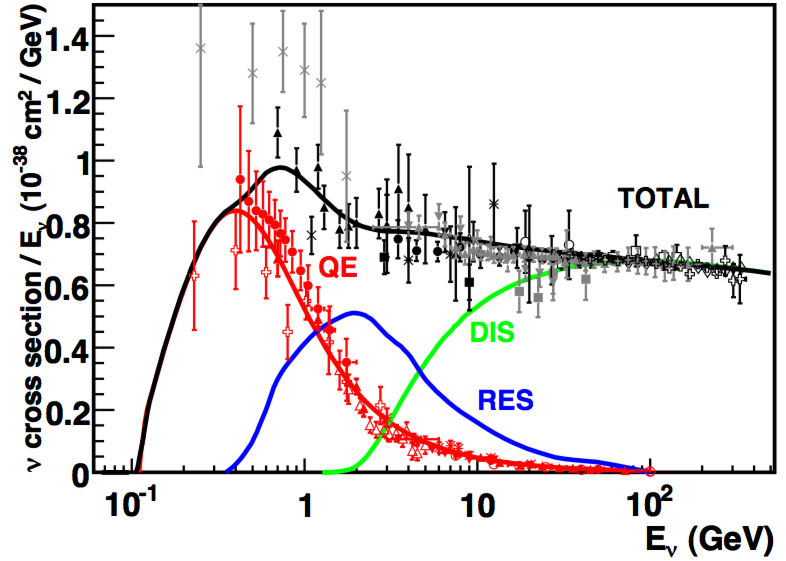
\includegraphics[width=6in]{Figures/neutrino-xsec.png}
\caption{The $\mu_\nu$ induced charged-current cross section measurements and the predictions as a function of neutrino energy \cite{Hewett:2012ns}. For reference, T2K has a peak muon neutrino energy of 600~MeV.} 
\label{fig:CCxsec}
\end{figure}

In the T2K neutrino beam energy regime, there are three major CC interaction channels that contribute to the total inclusive cross section: quasi-elastic (QE) scattering, resonant pion production and deep inelastic scattering. The cross sections of these neutrino-nucleon processes peak at different energy ranges as shown in Figure \ref{fig:CCxsec}. The theoretical calculation of the expressions modeling QE, resonance and DIS cross sections is extremely involved and has been developed over many decades. Even so, as the resolving power improves and amount of data increases, the models are undergoing continuous changes. We discuss the nature of the weak current, the general structure of the nucleon current and then summarize some of the more fundamental formulations of the three primary CC process cross sections.

\subsubsection{V-A Nature of the Weak Current}

In 1957, it was discovered that the weak interaction violated parity \cite{Wu:1957}, a rather surprising result at the time. To account for this in theory, the universal V-A theory of weak interactions was developed. To understand this, we first look at all the possible bilinear covariant expressions we can form out of the Dirac $\gamma$ matrices and a Dirac spinor $\psi$. There are only five independent expressions we can form from $\gamma$ matrices and they have definitive transformation properties under the Lorentz group and the parity operator. These five matrices along with their transformative properties are shown in Table \ref{tab:currpos} with $\gamma^5\equiv i \gamma^0 \gamma^1 \gamma^2 \gamma^3$.

\begin{table}[h]
\caption{List of all the possible independent bilinear covariant combinations of Dirac matrices along with the effect under Parity and Lorentz group transformations.}
\centering
\begin{tabular}{cccc}\toprule
Expression & \# of Component & Effect under Parity & Transformative Property\\
\midrule
$\overline{\psi}\psi$ & 1 & $+$ & Scalar \\
$\overline{\psi}\gamma^\mu \psi$ & 4 & $(+,-,-,-)$ & Vector \\
$\overline{\psi} \sigma^{\mu\nu} \psi = \frac{i}{2} \left[ \gamma^\mu , \gamma^\nu \right] $ & 6 & $ $ & Tensor \\
$\overline{\psi}\gamma^\mu \gamma^5 \psi$ & 4 & $(+,+,+,+)$ & Axial Vector \\
$\overline{\psi}\gamma^5 \psi$ & 1 & $-$ & Pseudo-Scalar \\ \bottomrule
\end{tabular} 
\label{tab:currpos}
\end{table}

Neutrinos are observed to be left-handed chiral particles, so given the left-handed chiral projection operator is $P_L = \frac{1}{2}\left( 1-\gamma^5\right)$, the current that is responsible for weak interactions should look like
\begin{equation}
\overline{\psi} \hat{O} P_L \phi
\end{equation}
where $\hat{O}$ is an operator that is a yet unknown combination of $\gamma$ matrices and $\phi$ is another Dirac spinor. Experimentation showed that $\hat{O}$ was simply $\gamma^\mu$, so the current explands to
\begin{equation}
\overline{\psi} \gamma^\mu \frac{1}{2}\left(1-\gamma^5\right) \phi = \frac{1}{2} \left(\overline{\psi}\gamma^\mu\phi - \overline{\psi} \gamma^\mu\gamma^5\phi\right).
\end{equation}

If we compare the two terms in this current with Table \ref{tab:currpos}, we find that first is a vector and the second is an axial vector. Therefore, the current describing weak interactions has the aforementioned V-A structure, a key realization in constructing an expression for the cross section of a CC interaction. The V-A structure implies parity violation as the vector and the axial parts transform differently under parity.

\subsubsection{Charge-Current Quasi-Elastic Cross Section}
\label{sec:ccqexsec}

We can now begin to study the theory behind neutrino-nucleon scattering by first looking at the $\nu_\mu$ quasielastic charged-current reaction
\begin{equation}
\nu_\mu + n \rightarrow p + \mu^{-}.
\end{equation}

\begin{figure}
\centering
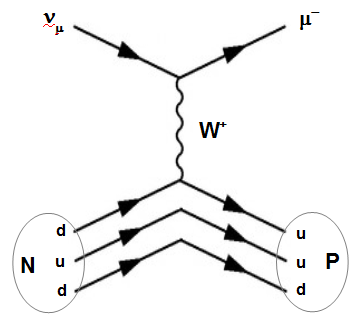
\includegraphics[width=3in]{Figures/ccqefeynman.png}
\caption{The lowest order Feynman diagram for the $\nu_\mu$ CCQE scattering process on a down quark. The W boson actually interacts with the neutron as a bound state of three quarks which significantly complicates the cross section calculation. Note that the general CCQE interaction could involve $\nu_e$ or $\nu_\tau$ instead of the $\nu_\mu$ lepton.} 
\label{fig:ccqefeynman}
\end{figure}

Charged current interactions can also occur with other leptons as well as anti-neutrinos, but as our beam consists almost entirely of muon neutrinos, we only study this particular interaction. Using the Feynman rules, we can construct the scattering amplitude for a neutrino with a down quark in the neutron for the first order process shown in Figure \ref{fig:ccqefeynman}. This expression, given the $d \rightarrow u$ transition, is \cite{GKbook}
\begin{equation}
\mathcal{A} = -i \frac{G_F}{\sqrt{2}}V_{ud}\left[\overline{u_\mu}(p_\mu)\gamma^\rho (1-\gamma^5)u_\nu(p_\nu)\right] \times \left[\overline{u_u}(p_u)\gamma^\rho(1-\gamma^5)u_d(p_d)\right]
\end{equation}
where the $u(p)$ terms are 4-vector representations of solutions to the Dirac equation corresponding to each of the external lines. The issue here is that the quarks are not free quarks as this expression would imply. Instead, they are bound into nucleons. So we replace the quark current with a \emph{nucleon current} to characterize the proper hadronic transition matrix:
\begin{equation}
\overline{u_u}(p_u)\gamma^\rho(1-\gamma^5)u_d(p_d) \rightarrow \bra{p(p_p)} h^\rho_W (0) \ket{n(p_n)}.
\end{equation}
The hadronic current is known to be of the form V-A as discussed before, so we split it into the vector and axial parts:
\begin{equation}
h^\rho_W (x) = v^\rho_W(x) - a^\rho_W(x).
\end{equation}
The vector and axial parts are now constructed separately by using the neutron 4-vector $p_n$ and the proton 4-vector $p_p$, the only kinematic variables available to us. Then, the most general hadronic vector matrix element possible is
\begin{equation}
\bra{p(p_p)} v^\rho_W(0)\ket{n(p_n)} = \overline{u_p}(p_p)\left[ f_1(q^2) \gamma^\rho + f_2(q^2)(p^\rho_n + p^\rho_p) + f_3(q^2)(p^\rho_n - p^\rho_p)\right] u_n(p_n)
\end{equation}
where $f_i(q^2)$ are form factors that are a function of the only scalar that can be constructed from $p_n$ and $p_p$:
\begin{equation}
p_n \cdot p_p = \frac{1}{2}\left[m_n^2 +m_p^2 -(p_p-p_n)^2\right] = \frac{1}{2}\left[m_n^2+m_p^2-q^2\right].
\end{equation}
We replace $p_p-p_n$ with $q$. The expression $Q^2 \equiv -q^2$ will also be used quite often in the formalism. As the mass terms are constant, the form factors are a function only of $q^2$. If $m_N \simeq m_n \simeq m_p $ and the Dirac equation is applied, the hadronic vector matrix element can be rewritten. The axial component can also be constructed following the same logic. The vector and axial components of the hadronic matrix element are 
\begin{align}
\bra{p(p_p)} v^\rho_W(0)\ket{n(p_n)} = & \overline{u_p}(p_p)\left[ \gamma^\rho F_1(Q^2) + \frac{i \sigma^{\rho\eta}q_\eta}{2 m_N} F_2(q^2) + \frac{q^\rho}{m_N}F_3(q^2)\right] u_n(p_n), \\
\bra{p(p_p)} a^\rho_W(0)\ket{n(p_n)} = & \overline{u_p}(p_p)\left[ \gamma^\rho \gamma^5 G_A(Q^2)  + \frac{q^\rho}{m_N} \gamma^5 G_P(q^2) + \frac{p^\rho_p+p^\rho_n}{m_N} \gamma^5 G_3(Q^2) \right] u_n(p_n).
\end{align}

The $F_3(Q^2)$ and $G_3(Q^2)$ terms, also known as second-class currents, have been confirmed to be zero by experimentation. The theory that suggested the disappearance of second-class currents involves the conservation of isovector current, also known as the conserved vector current (CVC) hypothesis, an important result. The remaining form factors $F_1(Q^2)$, $F_2(Q^2)$, $G_A(Q^2)$ and $G_P(Q^2)$ are called the Dirac, Fermi, axial and pseudo-scalar form factors respectively. These form factors essentially describe how a nucleon as a bound state of quarks is different from a point-like particle. Putting it all together, the scattering amplitude is 
\begin{multline}
\mathcal{A} = -i \frac{G_F}{\sqrt{2}}{V_{ud}}\left[\overline{u_\mu}(p_\mu)\gamma^\rho (1-\gamma^5)u_\nu(p_\nu)\right] \\ \times \left\{ \overline{u_p}(p_p)\left[ \gamma^\rho F_1(Q^2) + \frac{i \sigma^{\rho\eta}q_\eta}{2 m_N} F_2(q^2) +  \gamma^\rho \gamma^5 G_A(Q^2)  + \frac{q^\rho}{m_N} \gamma^5 G_P(q^2)\right] u_n(p_n) \right\}.
\end{multline}
Following the work of Llewellyn Smith \cite{LSCCQE}, this amplitude yields a $Q^2$ dependent differential cross section in the lab frame (nucleon at rest) of
\begin{equation}
\frac{d\sigma^{\nu_\mu n}_{CC}}{dQ^2} = \frac{G_F^2 |V_{ud}|^2 m_N^4}{8\pi (p_\nu \cdot p_N)^2} \left[ A(Q^2) + B(Q^2)\frac{s-u}{m_N^2} + C(Q^2)\frac{(s-u)^2}{m_N^4}\right],
\end{equation}
where $s$, $t$ and $u$ are the Mandelstam variables
\begin{align}
s \equiv & (p_\nu+p_N)^2,\\
t \equiv & (p_\nu+p_\mu)^2 = -Q^2,\\
u \equiv & (p_\mu+p_N)^2.
\end{align}
The $A(Q^2)$, $B(Q^2)$ and $C(Q^2)$ terms are written separately to clean up this rather messy cross section equation. They are given by

\begin{align}
\begin{split}
A = { }& \frac{m_\mu^2+Q^2}{m_N^2}\left\{\left( 1+\frac{Q^2}{4m_N^2}\right) G_A^2 - \left(1-\frac{Q^2}{4m_N^2}\right)\left(F_1^2-\frac{Q^2}{4m_N^2}F^2_2\right) + \frac{Q^2}{m_N^2}F_1 F_2\right. \nonumber\\
 &\left. - \frac{m_\mu^2}{4m_N^2}\left[(F_1+F_2)^2+(G_A+2G_P)^2 - \frac{1}{4}\left(1+\frac{Q^2}{4m_N^2}\right)G_P^2\right]\right\} ,
\end{split}\\
B = { }& \frac{Q^2}{m_N^2}G_A(F_1+F_2),\nonumber\\
C = { }& \frac{1}{4}\left(G_A^2+F_1^2+\frac{Q^2}{4m_N^2}F_2^2\right) .\nonumber
\end{align}
In the $A(Q^2)$ expression, $m_\mu^2 / m_N^2 \simeq 1.3\times10^{-2}$, so that entire term can be neglected for this particular scattering calculation. This also removes the dependence of the cross section on the $G_P$ form factor, leaving only $F_1$, $F_2$ and $G_A$. The axial form factor is parametrized as
\begin{equation}
G_A{Q^2} = \frac{g_A}{(1+Q^2/m_A^2)^2}.
\end{equation}
The $m_A$ term is called the \emph{axial mass} and has been determined by experiments to be $m_A = 1.026 \pm 0.021 GeV$. However, a $Q^2$ differential CCQE cross section measurement made by MiniBooNE \cite{MBCCQE}, a short-baseline neutrino experiment, suggested that the current value of $m_A$ determined from electron scattering might be too low. While there are suggested cross section modifications that fit the MiniBooNE data without altering the axial mass value, the T2K experiment accounts for the discrepancy by assigning a significant uncertainty to the CCQE $m_A$. Further CCQE cross section data fits will significantly improve our understanding of the nucleon form factors and determine the $m_A$ value from neutrino scattering.

Finally, as it is often possible to reconstruct the angle of the outgoing muon($\theta$) in a detector, it is practical to also calculate the angular differential cross-section in the lab frame:
\begin{equation}
\frac{d\sigma^{\nu_\mu n}_{CC}}{d\cos\theta} = -\frac{G_F^2 |V_{ud}|^2 m_N^2}{4\pi} \frac{p_\mu}{E_\nu}\left[ A(Q^2) + B(Q^2)\frac{s-u}{m_N^2} + C(Q^2)\frac{(s-u)^2}{m_N^4}\right].
\end{equation}
Here, assuming that the nucleon is at rest, $s-u = 4m_N E_\nu - 2 E_\nu (E_\mu - p_\mu \cos\theta)$. 

\subsubsection{Charged-Current Resonant Pion Production}
\label{sec:resxsec}

The next contributor to the total charged-current inclusive cross section is the resonant pion production process. A neutrino scatters off a nucleon, exciting it to a higher energy state and eventually decaying to a low multiplicity pion state in the following possible ways:
\begin{align}
\nu_\mu + p(n) &\rightarrow \mu^{-}+\pi^++p(n),\\
\nu_\mu + n &\rightarrow \mu^{-}+\pi^0+p.
\end{align}

\begin{figure}
\centering
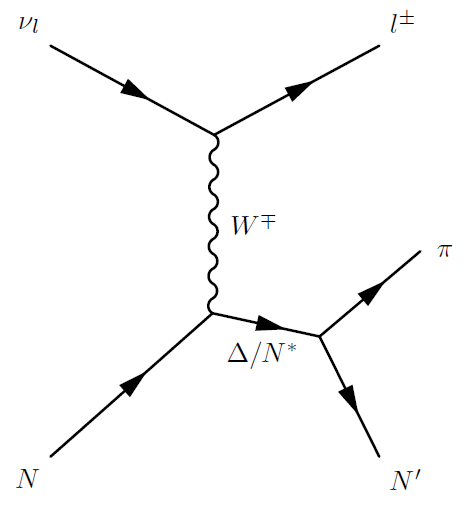
\includegraphics[width=3in]{Figures/1pi.png}
\caption{The Feynman diagram for the resonant scattering process on a nucleon. The neutrino excites the nucleon to a higher energy state which then decays to a single pion.} 
\label{fig:1pi}
\end{figure}
The Feynman diagram for these processes is generalized in Figure \ref{fig:1pi}. As the $Q^2$ is necessarily larger than in the CCQE interaction, this mode does not start to contribute significantly until 1~GeV neutrino energies. Rein and Sehgal \cite{RS1pi} have developed a model to describe the resonant cross section below 2~GeV. As the Rein-Sehgal model is used in the T2K simulation, we summarize their calculation here.

We begin with the Feynman rules to construct the expression for the invariant amplitude of charged-current resonance scattering. As before, the interaction is not on a free quark but on a bound quark in a nucleon, so we use a nucleon current expression instead of the quark current. Then, the invariant amplitude expression is 
\begin{equation}
\mathcal{A}(\nu N \rightarrow \mu N^*) = \frac{g^2 \cos\theta_C}{8}\left[ \overline{u_\mu} \gamma^\rho(1-\gamma^5) u_\nu \right] \left(\frac{g_{\rho\eta}-q_\rho q_\eta}{q^2-M_W^2}\right) \bra{N^*}J_\rho\ket{N}.
\end{equation}
In the accelerator experiment ranges of $|q^2| < 2~\text{GeV}$, terms of the form $|q^2|/M_W^2$ can be neglected. With the added simplifications of $G_F/\sqrt{2} = g^2/(8M_W^2)$ and $G_F \cos\theta_C \approx G_F$, the amplitude reduces to
\begin{equation}
\mathcal{A} = \frac{G_F}{\sqrt{2}}\left[ \overline{u_\mu} \gamma^\rho(1-\gamma^5) u_\nu \right] \bra{N^*}J_\rho\ket{N}.
\end{equation}
The lepton current can be considered as the W boson's polarization vector and is represented by three polarization vectors that correspond to left-handed, right-handed and scalar polarization components. In the frame where the virtual W boson momentum is in the positive Z direction, these polarization vectors are
\begin{align}
e^\rho_L &= \frac{1}{\sqrt{2}}(0, 1, -i, 0)\\
e^\rho_R &= \frac{1}{\sqrt{2}}(0, -1, -i, 0)\\
e^\rho_0 &= (1,0,0,0).
\end{align}
The lepton current can be simplified in the leptonic Breit frame,
\begin{equation}
\overline{u_\mu} \gamma^\rho(1-\gamma^5) u_\nu = -2\sqrt{2}\sqrt{-q^2}e^\rho_L,
\end{equation}
and then Lorentz boosted to the hadron Breit frame,
\begin{equation}
\overline{u_\mu} \gamma^\rho(1-\gamma^5) u_\nu = -\sqrt{2}\sqrt{-q^2}(1-\cosh \xi)e^\rho_L +(1-\cosh\xi)e^\rho_R + 2 \sinh\xi e^\rho_0,
\end{equation}
where the boost parameter $\xi$ is related to kinematical variables:
\begin{align}
\cosh\xi &= \frac{E_\nu^{lab} + E_\mu^{lab}}{|\vec{q}^{lab}|} \\
\sinh \xi &= \sqrt{\cosh^2\xi -1}.
\end{align}
For practical purposes, the leptonic current should be Lorentz boosted to the rest frame of the resonance. This transforms the scalar polarization vector to 
\begin{equation}
e^\rho_0 \rightarrow e^\rho_S= \frac{1}{\sqrt{-q^2}}(|\vec{q}|\frac{m_N}{M}, 0, 0, \sqrt{q^2+|\vec{q}|\frac{m_N^2}{M^2}}).
\end{equation}
This yields the lepton current expression in the resonance rest frame:
\begin{equation}
\overline{u_\mu} \gamma^\rho(1-\gamma^5) u_\nu = -2\sqrt{2}E^{lab}_\nu\sqrt{\frac{-q^2}{\vec{q^{lab}}^2}}(u\cdot e^\rho_L - v\cdot e^\rho_R + \sqrt{2uv}\cdot e^\rho_s),
\end{equation}
where
\begin{align}
u &= \frac{E_\nu^{lab}+E_\mu^{lab}+\vec{q}^{lab}}{2E^{lab}_\nu}\\
v &= \frac{E^{lab}_\nu+E^{lab}_\mu-\vec{q}^{lab}}{2E^{lab}_\nu}.
\end{align}
When the pieces of the lepton current are combined with the hadronic current, along with the identification $F_\rho = J_\rho/(2M)$, the invariant amplitude is
\begin{equation}
\mathcal{A} = -4GME\left[\sqrt{\frac{Q^2}{|\vec{q}|^2}} \bra{N^*} uF_- - vF_+ \ket{N} + \frac{m_N}{M}\sqrt{2uv}\bra{N^*}F_0\ket{N}\right],
\end{equation}
where
\begin{align}
F_+ &= e^\rho_R F_\rho = \frac{-1}{\sqrt{2}}(F_x+iF_y)\\
F_- &= e^\rho_L F_\rho = \frac{1}{\sqrt{2}}(F_x-iF_y)\\
F_0 &= \sqrt{\frac{Q^2}{|\vec{q}|^2}}e^\rho_S F_\rho = F_t+\frac{E_q}{|\vec{q}|}F_z.
\end{align}
This leads to a differential resonance cross section of
\begin{equation}
\frac{d\sigma}{dQ^2 dE_q} = \frac{1}{64\pi m_N E_\nu^2} \sum_{spins} |\mathcal{A}^2| \left(\frac{1}{2\pi}\cdot\frac{\Gamma}{(W-M)^2+\Gamma^2/4}\right)
\end{equation}
where the parenthesized term is simply the Breit-Wigner function with the resonance mass ($M$), the observed energy of the resonance ($W$) and the resonance width ($\Gamma$). The helicity terms in the amplitude
\begin{align}
f_{\pm} &= \bra{N}F_{\pm}\ket{N^*}\\
f_{0} &= \bra{N}F_{0}\ket{N^*}
\end{align}
are referred to as the helicity amplitudes. To calculate the overall resonance interaction cross section, the helicity amplitudes and the corresponding decay amplitude into a pion state for each single resonance are summed together. The isospin Clebsch-Gordan rules for the different isospin resonances yield the coefficients on each term being summed together. The decay amplitude of each single resonance is constructed by multiplying together the Breit-Wigner term, the decay sign and the square root of the resonance elasticity relating to the branching ratio of each pion state decay. 

To calculate the helicity and decay amplitudes, the dynamics of the nucleon must be defined somehow. Using the three bound quark model outlined by Feynman, Kislinger, and Ravandal \cite{FKR} (FKR), this task is possible. The FKR model depicts the quark Hamiltonian with a relativistic harmonic oscillator potential and has exhibited excellent predictive power in certain energy regimes. The FKR model proposes a four-dimensional Hamiltonian of the form
\begin{equation}
\mathcal{H} = 3(p_a^2+p_b^2+p_c^2)+\frac{1}{36}\Omega^2\left[(u_a-u_b)^2+(u_b-u_c)^2+(u_c-u_a)^2\right]+\text{const.}
\end{equation}
where $p_a$ is the four-momentum operator of quark a, $u_a$ is its conjugate position ($p_{a\mu} = i(\delta/\delta u_a^\mu$) and $\Omega$ is the spacing of energy levels per unit angular momentum. The calculation of the helicity amplitudes for each isospin resonance is quite involved and carried out in the FKR paper and the results are resummarized by Rein and Sehgal. The cross section expressions depend on vector and axial form factors $G_A$ and $G_V$ which take the dipole form
\begin{equation}
G^{V,A}(Q^2) = \left( 1+ \frac{Q^2}{4m_N^2}\right)^{1/2-n}\left(\frac{1}{1+Q^2/m_{V,A}^2}\right)^2.
\end{equation}
Electron scattering experiments have measured the vector mass, $m_V = 0.84$~GeV, while the axial mass, $m_A$ is yet to be fully constrained by neutrino experiments.

\subsubsection{Neutrino Deep Inelastic Scattering}
\label{sec:disxsec}

The final major process that contributes to the charged-current cross section in the $Q^2>>m_N$ energy transfer regime is deep inelastic scattering (DIS):
\begin{equation}
\nu_\mu + N \rightarrow \mu^{-}+X,
\end{equation}
where X is any number of other particles. 
%The Feynman diagram corresponding to this process is shown on the left in Figure \ref{fig:dis}.

%\begin{figure}
%\centering
%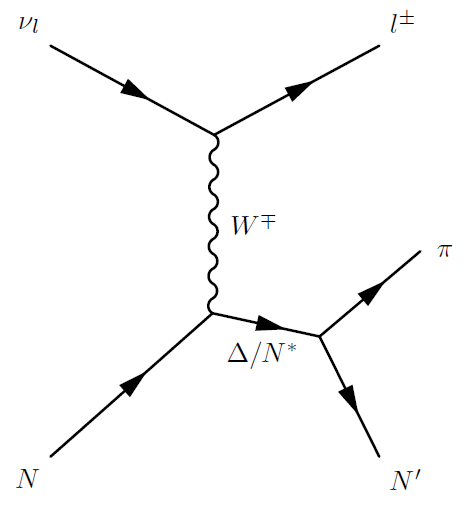
\includegraphics[width=6in]{Figures/1pi.png}
%\caption{(Left) The Feynman diagram for the deep inelastic scattering off a nucleon N. (Right) The same Feynman diagram adjusted to depict the nucleon scattering off a constituent down quark as described by the quark parton model (QPM).} 
%\label{fig:dis}
%\end{figure}

 The cross section is written \cite{GKbook} as a function of $Q^2\equiv -q^2$ and three other Lorentz-invariant kinematical variables: 
\begin{align}
s &= (p_\nu+p_N)^2 = m_N^2+2p_\nu\cdot p_N, \\
x &= \frac{Q^2}{2p_N\cdot q},\\
y &= \frac{p_N\cdot q}{p_N\cdot p_\nu}.
\end{align}
The differential DIS cross section is
\begin{equation}
\frac{d^2\sigma^{\nu N}_{CC}}{dx dy} = \frac{G_F^2}{2\pi}s \left(1+\frac{Q^2}{m_W^2}\right)^{-2}\left[x y^2 F_1 + (1-y)F_2 + xy\left(1-\frac{y}{2}\right)F_3 \right]
\end{equation}
where $F_i$ are called structure functions.

The quark parton model (QPM), originally developed by Feynman in 1969 \cite{QPM}, can be used to describe the structure functions in the DIS cross section. There are four basic assumptions in the QPM. First, a nucleon is made of a sea of quarks. 
%In this case, the neutrino is scattering off one of these quarks as depicted on the right in Figure \ref{fig:dis}. 
In this case, the neutrino is scattering off one of these quarks. Second, in the DIS regime, the quarks are asymptotically free, i.e. they do not interact with one another. Third, in the Breit frame where $|q^2| = -2 x \vec{p}_N$ and $|\vec{p}_N|^2 >> m_N^2$, the quarks all have three-momenta in the same direction. Finally, the quark masses can be neglected. Given these assumptions, the structure functions can be written in terms of what are known as the parton distribution functions (PDF), $f_q^N(x)$ which are probability densities of finding a quark, $q$, of four-momenta $p_i=x p_N$:

\begin{equation}
F_i(x) = \xi_i \sum_{q=d,s} f^N_q(x)+\overline{\xi_i} \sum_{\overline{q}=\overline{u},\overline{c}} f_{\overline{q}}^N(x)
%\overline{q}^N(x)
\end{equation}
with
\begin{equation}
\xi_1 = \overline{\xi_1} = 1, \xi_2=\overline{\xi_2}=2x, \xi_3=-\overline{\xi_3}=2.
\end{equation}
So finally, the double differential cross section for charged-current DIS is
\begin{equation}
\frac{d^2\sigma^{\nu N}_{CC}}{dx dy} = 2x \frac{G_F^2 m_N E_\nu}{\pi}\left[\sum_{q=d,s} f^N_q(x)+(1-y)^2 \sum_{\overline{q}=\overline{u},\overline{c}}f_{\overline{q}}^N(x)\right].
\end{equation}

\subsubsection{Nuclear Effects}

Similar to how quasi-elastic scattering conducted on a free quark is too simplistic a picture of the process, neutrino-nucleon scattering is also a simplification of the actual case. In reality, the proton and neutrons are not free but bound in a nucleus. This necessitates the modeling of nuclear level effects. The current model of nucleons is as a relativistic fermi gas (RFG) \cite{RFG}. They are given a flat momentum density below the Fermi momentum limit $p_F$. There are however other models that may prove an improvement. In one such mode, the RFG density of states is replaced by a ``spectral function" that is a probability distribution of finding a nucleon with a momentum and a removal energy \cite{SF}.

Another issue is the current tension between CCQE cross section data from the MiniBooNE experiment and older experiments such as NOMAD. Under the Lewellyn-Smith model, a single value of the axial mass does not fit the cross section vs. $Q^2$ distributions of both experiments. In our analysis, we account for this tension by inflating the errors applied to the global best fit value of the axial mass. However, there are other models currently under investigation. For example, the ``multinucleon effect" considers the corrections required when a neutrino interacts with a correlated pair of nucleons instead of a single, free nucleon. While the physics simulation used in our analysis does not include such corrections, the multinucleon effect has made great strides towards reconciling the MiniBooNE and NOMAD CCQE cross section measurements.

Other than nucleon momenta modeling, there are also intra-nuclear effects on produced particles as they exit. Pions produced via resonance can interact with the nuclear medium and be absorbed or neutralized. A cascade model is used by T2K to attempt to correct for these intra-nuclear effects though as we will find, the effect on an inclusive measurement is rather small. 
